\chapter{Fuerzas intermoleculares y disolventes}\label{ch:b1:intermolecular-forces-solvents}

Un geco sube corriendo por el cristal de una ventana y se queda colgado
de un solo dedo; sin pegamento ni ventosas, solo con la atracción entre
las moléculas de las almohadillas de sus dedos y las del vidrio. El agua,
una molécula más ligera que el dióxido de carbono, hierve a
\qty{100}{\celsius}, mientras que el dióxido de carbono es un gas a
temperatura ambiente. El aceite flota sobre el vinagre y nunca se mezcla
con él; la sal de mesa se disuelve en el agua y no en la gasolina. Todos
estos hechos no los deciden los enlaces del interior de las moléculas,
sino las fuerzas, mucho más débiles, que actúan entre ellas. Este capítulo
clasifica esas fuerzas, mide sus efectos sobre las temperaturas de
ebullición y las utiliza para elegir un disolvente.

% ledger: bp:H2O (the hook's 100 degC)

\begin{recall}
El libro 1 (año 11) introdujo las fuerzas de van der Waals y los \omterm{def:b1:intermolecular-forces-solvents:hbond}{enlaces
de hidrógeno}, y explicó que los sólidos iónicos se disuelven por
disociación y \omterm{def:b1:intermolecular-forces-solvents:dissolution}{solvatación}. Los \omterm{def:b1:lewis-resonance-vsepr:dipole}{momentos dipolares} se definieron en la
\cref{def:b1:lewis-resonance-vsepr:dipole}, y la \omterm{def:b1:periodicity:polarisability}{polarizabilidad}, en la
\cref{def:b1:periodicity:polarisability}. De la física se usa la ley de
Coulomb: dos cargas $q_1$ y $q_2$ a una distancia $r$ en el vacío se
atraen o se repelen con una fuerza de norma $|q_1q_2|/(4\pi
\varepsilon_0 r^2)$.
\end{recall}

\begin{omfigure}
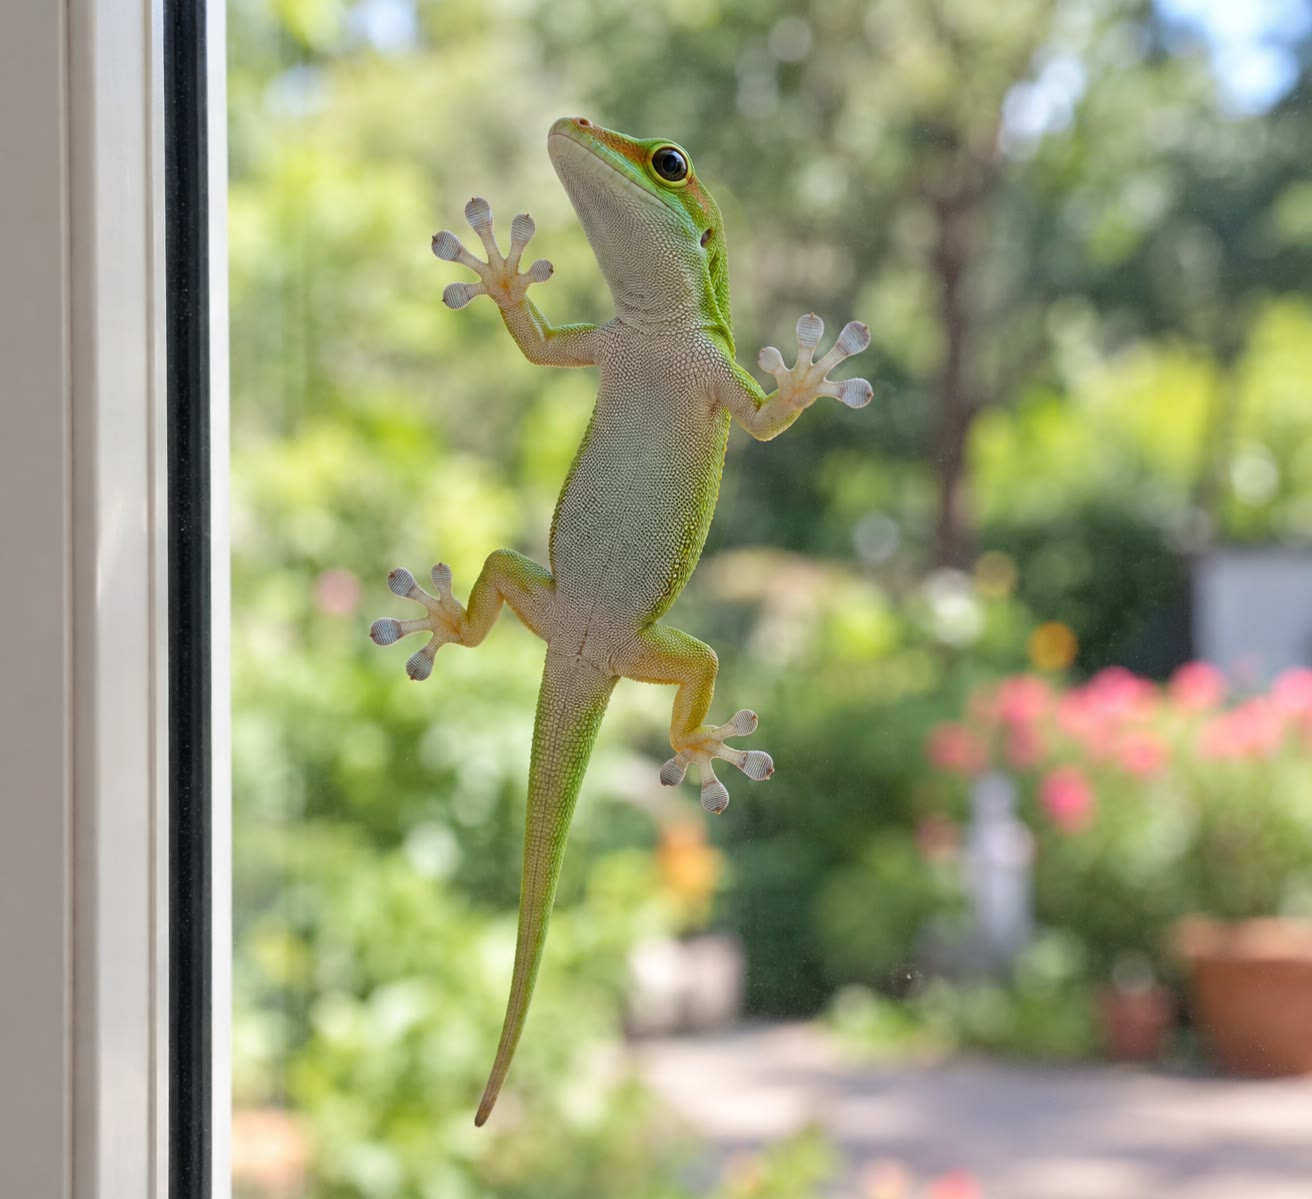
\includegraphics[width=0.52\linewidth]{images/book2/ai/b1-04-gecko.jpg}

{\small Un geco en el cristal de una ventana. Los millones de finísimos
pelos de las almohadillas de sus dedos se acercan tanto al vidrio que la
débil atracción entre sus moléculas y las del vidrio llega a superar su
peso.}
\end{omfigure}

\section{Interacciones de van der Waals}

\begin{definition}[Interacciones de van der Waals]\label{def:b1:intermolecular-forces-solvents:vdw}
Las \emph{interacciones de van der Waals}\index{interaccion de van der Waals@interacción de van der Waals}
son las atracciones entre moléculas neutras que proceden de la
interacción de sus dipolos. Se distinguen tres tipos:
\begin{itemize}
  \item la \emph{interacción de Keesom}\index{interaccion de Keesom@interacción de Keesom} (o
        interacción de orientación), entre dos dipolos permanentes, que
        tienden a alinearse uno tras otro;
  \item la \emph{interacción de Debye}\index{interaccion de Debye@interacción de Debye} (o
        interacción de inducción), entre un dipolo permanente y el dipolo
        que induce en un vecino polarizable;
  \item la \emph{interacción de London}\index{interaccion de London@interacción de London} (o
        interacción de dispersión), entre los dipolos instantáneos que
        las fluctuaciones de las nubes electrónicas crean en dos átomos o
        moléculas cualesquiera, polares o no, y que se inducen
        mutuamente.
\end{itemize}
\end{definition}

\begin{omfigure}
\begin{tikzpicture}[font=\small, >={Stealth},
    mol/.style={draw=black!60, fill=#1, ellipse, minimum width=1.5cm, minimum height=0.8cm}]
  % Keesom
  \node[mol=omDef!20] (a) at (0,0) {}; \node[mol=omDef!20] (b) at (1.7,0) {};
  \node at (-0.45,0) {$\delta^-$}; \node at (0.45,0) {$\delta^+$};
  \node at (1.25,0) {$\delta^-$}; \node at (2.15,0) {$\delta^+$};
  \node[below, align=center] at (0.85,-0.65) {Keesom:\\dos dipolos permanentes};
  % Debye
  \begin{scope}[xshift=4.6cm]
    \node[mol=omDef!20] at (0,0) {}; \node[mol=black!5, dashed] at (1.7,0) {};
    \node at (-0.45,0) {$\delta^-$}; \node at (0.45,0) {$\delta^+$};
    \node[omProp] at (1.25,0) {$\delta^-$}; \node[omProp] at (2.15,0) {$\delta^+$};
    \node[below, align=center] at (0.85,-0.65) {Debye:\\permanente e inducido};
  \end{scope}
  % London
  \begin{scope}[xshift=9.2cm]
    \node[mol=black!5, dashed] at (0,0) {}; \node[mol=black!5, dashed] at (1.7,0) {};
    \node[omProp] at (-0.45,0) {$\delta^-$}; \node[omProp] at (0.45,0) {$\delta^+$};
    \node[omProp] at (1.25,0) {$\delta^-$}; \node[omProp] at (2.15,0) {$\delta^+$};
    \node[below, align=center] at (0.85,-0.65) {London:\\dos dipolos instantáneos};
  \end{scope}
\end{tikzpicture}

{\small Las tres \omterm{def:b1:intermolecular-forces-solvents:vdw}{interacciones de van der Waals}. Las cargas parciales en
negro son permanentes (\omterm{def:b1:lewis-resonance-vsepr:dipole}{moléculas polares}); las naranjas son inducidas o
instantáneas. En los tres casos, las cargas enfrentadas son opuestas, de
modo que las moléculas se atraen.}
\end{omfigure}

\begin{proposition}[Intensidad y alcance]\label{prop:b1:intermolecular-forces-solvents:distance-law}
Para dos moléculas a una distancia $r$, cada una de las tres energías de
van der Waals varía como $-1/r^6$: la atracción solo se percibe entre
vecinos. Sus energías son del orden de unos pocos kilojulios por mol,
unas cien veces menos que un \omterm{def:b1:lewis-resonance-vsepr:lewis}{enlace covalente}. El término de London
crece con las \omterm{def:b1:periodicity:polarisability}{polarizabilidades} de los dos participantes; está presente
entre todas las moléculas y suele ser el mayor de los tres, salvo en
moléculas pequeñas y muy polares.
\end{proposition}
\admitted

\begin{example}[Gases nobles y halógenos]\label{ex:b1:intermolecular-forces-solvents:noble}
Los átomos de un gas noble solo se atraen por fuerzas de London, que
crecen con el número de electrones: el helio hierve a
\qty{-268.9}{\celsius}; el neón, a \qty{-246.1}{\celsius}; el argón, a
\qty{-185.9}{\celsius}; el criptón, a \qty{-153.4}{\celsius}, y el xenón,
a \qty{-108.1}{\celsius}. Del mismo modo, a temperatura ambiente, el
diflúor y el dicloro son gases; el dibromo, un líquido (que hierve a
\qty{58.8}{\celsius}), y el diyodo, un sólido.
% ledger: bp:He, bp:Ne, bp:Ar, bp:Kr, bp:Xe, bp:F2, bp:Cl2, bp:Br2, bp:I2
\end{example}

\begin{omfigure}
\begin{tikzpicture}
\begin{axis}[
  width=0.62\linewidth, height=5.4cm,
  xmin=0.5, xmax=10.5, ymin=-180, ymax=200,
  axis x line=bottom, axis y line=left,
  xlabel={número de átomos de carbono $n$}, ylabel={temperatura de ebullición (\unit{\celsius})},
  xtick={1,2,3,4,5,6,7,8,9,10}, ytick={-150,-100,-50,0,50,100,150},
  tick label style={font=\small}, label style={font=\small}]
\addplot[omDef, thick, mark=*, mark size=1.5pt] table[x=n, y=bp_C] {figdata/out/bachelor-1-hydride-boiling-points-alkanes.dat};
\end{axis}
\end{tikzpicture}

{\small Temperaturas de ebullición de los alcanos lineales
\ce{C_nH_{2n+2}}, del metano al decano. Cada \ce{CH2} añadido aporta
electrones y superficie de contacto y, por tanto, atracción de London;
el incremento disminuye lentamente, de unos \qty{75}{\celsius} al
principio a \qty{25}{\celsius} en el decano.}
\end{omfigure}

\section{El enlace de hidrógeno}

\begin{definition}[Enlace de hidrógeno]\label{def:b1:intermolecular-forces-solvents:hbond}
Un \emph{enlace de hidrógeno}\index{enlace de hidrogeno@enlace de hidrógeno} es una atracción
$\ce{X-H}\cdots\ce{Y}$ entre un átomo de hidrógeno unido a un átomo X
pequeño y muy electronegativo (\ce{N}, \ce{O} o \ce{F}) y un \omterm{def:b1:lewis-resonance-vsepr:lewis}{par no
enlazante} de otro átomo electronegativo Y. La molécula que lleva \ce{X-H}
es el dador del enlace de hidrógeno, y la que lleva Y, el aceptor. Su
energía, de 10 a \qty{40}{kJ/mol}, está entre la de las \omterm{def:b1:intermolecular-forces-solvents:vdw}{interacciones de
van der Waals} y la de los \omterm{def:b1:lewis-resonance-vsepr:lewis}{enlaces covalentes}; los tres átomos \ce{X},
\ce{H} e \ce{Y} están casi alineados.
\end{definition}

\begin{remark}[Por qué N, O y F]\label{rem:b1:intermolecular-forces-solvents:why}
Un X muy electronegativo deja al hidrógeno con una carga parcial positiva
grande; el hidrógeno, que no tiene \omterm{def:b1:quantum-numbers:configuration}{electrones internos}, es diminuto, de
modo que el \omterm{def:b1:lewis-resonance-vsepr:lewis}{par no enlazante} de Y puede acercarse mucho a él. Hacen falta
las dos condiciones: los enlaces \ce{C-H} no son lo bastante polares, y
los enlaces \ce{S-H} o \ce{Cl-H} implican átomos demasiado grandes y
demasiado poco electronegativos para formar \omterm{def:b1:intermolecular-forces-solvents:hbond}{enlaces de hidrógeno} fuertes.
\end{remark}

\begin{omfigure}
\begin{tikzpicture}[font=\small]
  % water network
  \foreach \n/\x/\y/\a in {1/0/0/0, 2/2.2/0.9/200, 3/0.2/-2.0/60, 4/-2.1/0.6/-30} {
    \begin{scope}[shift={(\x,\y)}, rotate=\a]
      \node[aO] (o\n) at (0,0) {};
      \node[aH] (h\n a) at (0.78,0.3) {};
      \node[aH] (h\n b) at (-0.2,-0.82) {};
      \begin{scope}[on background layer]
        \draw[bond] (o\n.center) -- (h\n a.center); \draw[bond] (o\n.center) -- (h\n b.center);
      \end{scope}
    \end{scope}
  }
  \draw[omThm, thick, densely dotted] (h1a) -- (o2);
  \draw[omThm, thick, densely dotted] (h1b) -- (o3);
  \draw[omThm, thick, densely dotted] (h4a) -- (o1);
  \node[below] at (0,-2.9) {agua: cada molécula puede dar dos y aceptar dos};
  % carboxylic acid dimer
  \begin{scope}[xshift=5.6cm, yshift=-0.6cm]
    \node (r1) at (-0.9,0) {R}; \node (c1) at (0,0) {C};
    \node (o1) at (0.6,0.85) {O}; \node (o2) at (0.6,-0.85) {O}; \node (h2) at (1.45,-0.85) {H};
    \node (c2) at (3.3,0) {C}; \node (r2) at (4.2,0) {R};
    \node (o3) at (2.7,0.85) {O}; \node (o4) at (2.7,-0.85) {O}; \node (h3) at (1.85,0.85) {H};
    \draw (r1) -- (c1) -- (o2) -- (h2) (c2) -- (r2) (c2) -- (o3) -- (h3);
    \draw[double, double distance=1.6pt] (c1) -- (o1); \draw[double, double distance=1.6pt] (c2) -- (o4);
    \draw[omThm, thick, densely dotted] (h2) -- (o4) (h3) -- (o1);
    \node[below] at (1.65,-2.3) {un dímero de ácido carboxílico};
  \end{scope}
\end{tikzpicture}

{\small \omterm{def:b1:intermolecular-forces-solvents:hbond}{Enlaces de hidrógeno} (en rojo, de puntos). En el agua líquida cada
molécula participa en hasta cuatro de ellos; los ácidos carboxílicos se
emparejan en dímeros cíclicos unidos por dos \omterm{def:b1:intermolecular-forces-solvents:hbond}{enlaces de hidrógeno}.}
\end{omfigure}

\begin{proposition}[Los enlaces de hidrógeno elevan la temperatura de ebullición]\label{prop:b1:intermolecular-forces-solvents:hbond-bp}
Entre los hidruros de los \omterm{def:b1:periodicity:table}{grupos} 15, 16 y 17, la temperatura de ebullición
aumenta del \omterm{def:b1:periodicity:table}{periodo} 3 al \omterm{def:b1:periodicity:table}{periodo} 5, siguiendo la \omterm{def:b1:intermolecular-forces-solvents:vdw}{interacción de London};
los hidruros del \omterm{def:b1:periodicity:table}{periodo} 2, \ce{NH3}, \ce{H2O} y \ce{HF}, que forman
\omterm{def:b1:intermolecular-forces-solvents:hbond}{enlaces de hidrógeno}, hierven muy por encima de la extrapolación de esa
tendencia. Los hidruros del \omterm{def:b1:periodicity:table}{grupo} 14 (\ce{CH4}, \ce{SiH4}, \ce{GeH4}) no
forman \omterm{def:b1:intermolecular-forces-solvents:hbond}{enlaces de hidrógeno} y siguen la tendencia.
\end{proposition}

\begin{omfigure}
\begin{tikzpicture}
\begin{axis}[
  width=0.82\linewidth, height=6.6cm,
  xmin=1.5, xmax=5.6, ymin=-180, ymax=120,
  axis x line=bottom, axis y line=left,
  xlabel={periodo}, ylabel={temperatura de ebullición (\unit{\celsius})},
  xtick={2,3,4,5}, ytick={-150,-100,-50,0,50,100},
  tick label style={font=\small}, label style={font=\small},
  clip=false]
\addplot[black!60, thick, mark=square*, mark size=1.6pt] table[x=period, y=bp_C] {figdata/out/bachelor-1-hydride-boiling-points-g14.dat};
\addplot[omDef, thick, mark=*, mark size=1.6pt] table[x=period, y=bp_C] {figdata/out/bachelor-1-hydride-boiling-points-g15.dat};
\addplot[omThm, thick, mark=*, mark size=1.6pt] table[x=period, y=bp_C] {figdata/out/bachelor-1-hydride-boiling-points-g16.dat};
\addplot[omMeth, thick, mark=triangle*, mark size=2pt] table[x=period, y=bp_C] {figdata/out/bachelor-1-hydride-boiling-points-g17.dat};
\addplot[omThm, dashed] coordinates {(2,-79.3) (3,-60.3)};
\node[font=\small, anchor=west] at (axis cs:2.05,100) {\ce{H2O}};
\node[font=\small, anchor=west] at (axis cs:2.05,19.6) {\ce{HF}};
\node[font=\small, anchor=west] at (axis cs:2.05,-30) {\ce{NH3}};
\node[font=\small, anchor=east] at (axis cs:1.96,-162) {\ce{CH4}};
\node[font=\small, anchor=west] at (axis cs:4.05,-41.3) {\ce{H2Se}};
\node[font=\small, anchor=west] at (axis cs:5.05,-18.4) {\ce{SbH3}};
\node[font=\small, anchor=west] at (axis cs:5.05,-35.1) {\ce{HI}};
\node[font=\small, anchor=west] at (axis cs:4.05,-88.1) {\ce{GeH4}};
\node[font=\small, omThm, anchor=north west] at (axis cs:2.05,-85) {extrapolado};
\end{axis}
\end{tikzpicture}

{\small Temperaturas de ebullición de los hidruros de los \omterm{def:b1:periodicity:table}{grupos} 14
(cuadrados grises), 15 (azul), 16 (rojo) y 17 (verde). El agua herviría
hacia \qty{-79}{\celsius} si siguiera a sus análogos más pesados
(discontinua); sus \omterm{def:b1:intermolecular-forces-solvents:hbond}{enlaces de hidrógeno} la elevan unos \qty{180}{\celsius}.}
% ledger: bp:CH4, bp:SiH4, bp:GeH4, bp:NH3, bp:PH3, bp:AsH3, bp:SbH3,
% bp:H2O, bp:H2S, bp:H2Se, bp:HF, bp:HCl, bp:HBr, bp:HI
\end{omfigure}

\begin{example}[El etanol y su isómero]\label{ex:b1:intermolecular-forces-solvents:isomers}
El etanol, \ce{CH3CH2OH}, y el metoximetano, \ce{CH3OCH3}, tienen la
misma fórmula, \ce{C2H6O}, y casi las mismas \omterm{def:b1:intermolecular-forces-solvents:vdw}{interacciones de London}. El
etanol, cuyo grupo \ce{O-H} es a la vez dador y aceptor, hierve a
\qty{78.4}{\celsius}; el metoximetano, que solo puede aceptar, hierve a
\qty{-25.0}{\celsius}.
% ledger: bp:C2H5OH, bp:CH3OCH3
\end{example}

\section{Disolventes}

\begin{definition}[Permitividad relativa]\label{def:b1:intermolecular-forces-solvents:permittivity}
En un medio, la fuerza de Coulomb entre dos cargas queda dividida por un
número $\varepsilon_r \ge 1$, la \emph{permitividad relativa}\index{permitividad relativa}
(o constante dieléctrica) del medio:
\[
  F = \frac{|q_1 q_2|}{4\pi\varepsilon_0\varepsilon_r r^2} .
\]
Es grande en los líquidos de \omterm{def:b1:lewis-resonance-vsepr:dipole}{moléculas polares}, que se orientan alrededor
de las cargas y las apantallan: \num{78.4} para el agua a
\qty{25}{\celsius} y \num{1.89} para el hexano a \qty{20}{\celsius}.
% ledger: epsr:H2O, epsr:C6H14
\end{definition}

\begin{definition}[Disolventes polares, próticos y apróticos]\label{def:b1:intermolecular-forces-solvents:solvent-classes}
Un \emph{disolvente polar}\index{disolvente polar} está formado por
moléculas de \omterm{def:b1:lewis-resonance-vsepr:dipole}{momento dipolar} grande y tiene una \omterm{def:b1:intermolecular-forces-solvents:permittivity}{permitividad relativa}
grande (superior a unos 15); un disolvente apolar la tiene pequeña. Un
\emph{disolvente prótico}\index{disolvente protico@disolvente prótico} tiene moléculas con
átomos de hidrógeno capaces de formar \omterm{def:b1:intermolecular-forces-solvents:hbond}{enlaces de hidrógeno} (\ce{O-H} o
\ce{N-H}); un \emph{disolvente aprótico}\index{disolvente aprotico@disolvente aprótico} no los
tiene.
\end{definition}

\begin{center}
\small
\begin{tabular}{lccll}
\hline
disolvente & $\varepsilon_r$ & $\mu$ (D) & polaridad & carácter prótico \\
\hline
agua & 78.4 & 1.86 & polar & prótico \\
metanol & 32.6 & 1.67 & polar & prótico \\
etanol & 24.3 & 1.52 & polar & prótico \\
acetonitrilo, \ce{CH3CN} & 37.5 & 3.92 & polar & aprótico \\
propanona (acetona) & 20.7 & 2.88 & polar & aprótico \\
diclorometano & 9.08 & 1.62 & poco polar & aprótico \\
etanoato de etilo & 6.02 & 1.78 & poco polar & aprótico \\
etoxietano & 4.34 & 1.15 & poco polar & aprótico \\
benceno & 2.28 & 0 & apolar & aprótico \\
hexano & 1.89 & 0 & apolar & aprótico \\
\hline
\end{tabular}
\end{center}
% ledger: epsr:H2O, epsr:CH3OH, epsr:C2H5OH, epsr:CH3CN, epsr:CH3COCH3,
% epsr:CH2Cl2, epsr:EtOAc, epsr:Et2O, epsr:C6H6, epsr:C6H14, dip:H2O,
% dip:CH3OH, dip:C2H5OH, dip:CH3CN, dip:CH3COCH3, dip:CH2Cl2, dip:EtOAc,
% dip:Et2O, dip:C6H6 (relative permittivities at 20 or 25 degC; dipole
% moments of the gas-phase molecules; hexane has no dipole by symmetry)

\begin{definition}[Solvatación, poder ionizante y poder disociante]\label{def:b1:intermolecular-forces-solvents:dissolution}
La \emph{solvatación}\index{solvatacion@solvatación} de una partícula de soluto es su
rodeamiento por moléculas de disolvente orientadas y unidas a ella por
fuerzas intermoleculares (hidratación, en el agua). El \emph{poder
ionizante}\index{poder ionizante} de un disolvente es su capacidad para
convertir un \omterm{def:b1:lewis-resonance-vsepr:lewis}{enlace covalente} polar del soluto en un par de iones,
propiedad de los \omterm{def:b1:intermolecular-forces-solvents:solvent-classes}{disolventes polares} de \omterm{def:b1:lewis-resonance-vsepr:dipole}{momento dipolar} grande; su
\emph{poder disociante}\index{poder disociante} es su capacidad para
separar los iones de un par, y se mide por su \omterm{def:b1:intermolecular-forces-solvents:permittivity}{permitividad relativa}.
\end{definition}

\begin{proposition}[La disolución en tres etapas]\label{prop:b1:intermolecular-forces-solvents:steps}
La disolución de un electrolito en un disolvente puede describirse en
tres etapas: ionización (para un soluto molecular como \ce{HCl}),
disociación de los pares de iones y \omterm{def:b1:intermolecular-forces-solvents:dissolution}{solvatación} de los iones separados.
Un disolvente disuelve bien un soluto iónico o muy polar cuando es polar
(ionizante), de permitividad alta (disociante) y capaz de solvatar los
dos iones --- los cationes con sus \omterm{def:b1:lewis-resonance-vsepr:lewis}{pares no enlazantes}, y los aniones con
\omterm{def:b1:intermolecular-forces-solvents:hbond}{enlaces de hidrógeno} si es prótico. El agua hace las tres cosas.
\end{proposition}

\begin{example}[El cloruro de hidrógeno en agua y en hexano]\label{ex:b1:intermolecular-forces-solvents:hcl}
En el agua, \ce{HCl} se ioniza y se disocia por completo:
\ce{HCl(g) + H2O(l) -> H3O+(aq) + Cl-(aq)}; la disolución conduce. En el
hexano, apolar y de baja permitividad, se disuelve en forma de moléculas
de \ce{HCl} y la disolución no conduce.
\end{example}

\begin{omfigure}
\begin{tikzpicture}[font=\small]
  \node[aNa] (na) at (0,0) {};
  \node[font=\scriptsize, white] at (na) {\ce{Na+}};
  \foreach \a in {0,60,...,300} {
    \begin{scope}[shift={(\a:1.25)}, rotate=\a]
      \node[aO] (o) at (0,0) {};
      \node[aH] (ha) at (0.55,0.5) {}; \node[aH] (hb) at (0.55,-0.5) {};
      \begin{scope}[on background layer]
        \draw[bond] (o.center) -- (ha.center); \draw[bond] (o.center) -- (hb.center);
      \end{scope}
    \end{scope}
  }
  \node[below] at (0,-2.4) {catión: pares del O hacia dentro};
  \begin{scope}[xshift=6.2cm]
    \node[aCl] (cl) at (0,0) {};
    \node[font=\scriptsize, white] at (cl) {\ce{Cl-}};
    \foreach \a in {0,60,...,300} {
      \begin{scope}[shift={(\a:1.55)}, rotate=\a]
        \node[aH] (h1) at (-0.62,0) {};
        \node[aO] (o) at (0,0) {};
        \node[aH] (h2) at (0.25,0.72) {};
        \begin{scope}[on background layer]
          \draw[bond] (o.center) -- (h1.center); \draw[bond] (o.center) -- (h2.center);
        \end{scope}
      \end{scope}
    }
    \node[below] at (0,-2.4) {anión: enlaces de H hacia dentro};
  \end{scope}
\end{tikzpicture}

{\small Hidratación de los dos iones del cloruro de sodio (solo la primera
capa, dibujada en el plano). El agua orienta su extremo negativo, el
oxígeno, hacia el catión, y un hidrógeno hacia el anión.}
\end{omfigure}

\section{Solubilidad, miscibilidad y anfífilos}

\begin{proposition}[Lo semejante disuelve a lo semejante]\label{prop:b1:intermolecular-forces-solvents:like}
Un soluto se disuelve bien en un disolvente cuando las interacciones
entre las moléculas de soluto y de disolvente son comparables a las que
pierden: los solutos polares o que forman iones, en \omterm{def:b1:intermolecular-forces-solvents:solvent-classes}{disolventes polares};
los solutos apolares, en disolventes apolares; los solutos que forman
\omterm{def:b1:intermolecular-forces-solvents:hbond}{enlaces de hidrógeno}, en \omterm{def:b1:intermolecular-forces-solvents:solvent-classes}{disolventes próticos}.
\end{proposition}

\begin{proof}[Razonamiento]
Disolver rompe interacciones soluto--soluto y disolvente--disolvente y
crea interacciones soluto--disolvente. Si el soluto es apolar y el
disolvente es agua, las moléculas de agua pierden \omterm{def:b1:intermolecular-forces-solvents:hbond}{enlaces de hidrógeno}
para hacerle sitio y solo ganan a cambio débiles \omterm{def:b1:intermolecular-forces-solvents:vdw}{interacciones de London}:
la disolución es desfavorable. Si ambos son apolares, las \omterm{def:b1:intermolecular-forces-solvents:vdw}{interacciones
de London} perdidas y ganadas son comparables, y la mezcla se ve
favorecida por el desorden que crea.
\end{proof}

\begin{definition}[Líquidos miscibles]\label{def:b1:intermolecular-forces-solvents:miscibility}
Dos líquidos son \emph{miscibles}\index{miscible} cuando se mezclan en
cualquier proporción en una sola fase líquida; si no, forman dos capas,
con la menos densa arriba.
\end{definition}

\begin{example}[Agua con etanol, agua con hexano]\label{ex:b1:intermolecular-forces-solvents:miscible}
El etanol es \omterm{def:b1:intermolecular-forces-solvents:miscibility}{miscible} con el agua: ambos son próticos y polares, y el
etanol forma \omterm{def:b1:intermolecular-forces-solvents:hbond}{enlaces de hidrógeno} con el agua igual que consigo mismo.
El hexano y el agua son inmiscibles. El diyodo, un sólido molecular, es
muy poco soluble en agua, pero se disuelve fácilmente en hexano o en
diclorometano: al agitar el yodo acuoso con uno de esos disolventes, pasa
a la capa orgánica, el principio de la extracción líquido--líquido
(\cref{ch:b1:lab-techniques-1}).
\end{example}

\begin{omfigure}
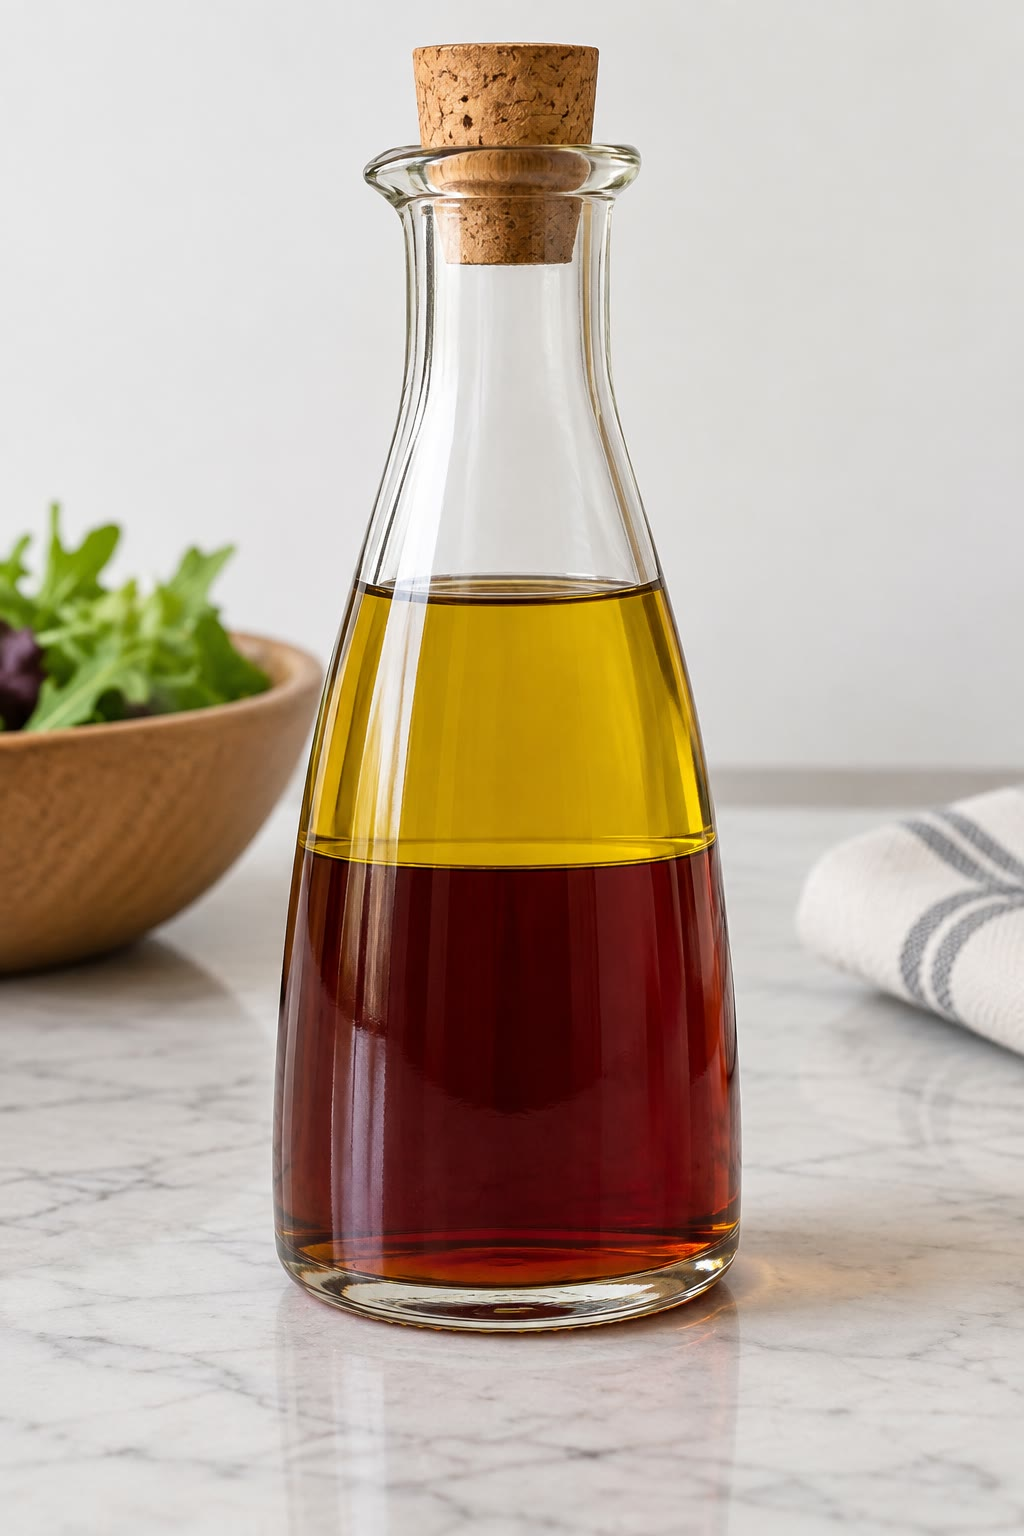
\includegraphics[width=0.2\linewidth]{images/book2/ai/b1-04-dressing.jpg}

{\small Una vinagreta en reposo: el aceite de oliva, apolar, flota sobre
el vinagre, una disolución acuosa; los dos líquidos son inmiscibles.}
\end{omfigure}

\begin{definition}[Hidrófilo, hidrófobo, anfífilo]\label{def:b1:intermolecular-forces-solvents:amphiphile}
Un grupo es \emph{hidrófilo}\index{hidrofilo@hidrófilo} cuando interactúa
favorablemente con el agua (grupos iónicos o polares: \ce{-COO^-},
\ce{-OH}, \ce{-SO3^-}) e \emph{hidrófobo}\index{hidrofobo@hidrófobo} cuando no lo hace
(cadenas hidrocarbonadas). Una molécula es
\emph{anfífila}\index{anfifila@anfífila} cuando lleva a la vez una cabeza hidrófila y
una cola hidrófoba.
\end{definition}

\begin{example}[El jabón]\label{ex:b1:intermolecular-forces-solvents:soap}
El dodecanoato de sodio, \ce{CH3(CH2)10COO- Na+}, es \omterm{def:b1:intermolecular-forces-solvents:amphiphile}{anfífilo}. En la
superficie del agua, sus moléculas se colocan con la cabeza en el agua y
la cola en el aire. En el seno del líquido, por encima de una pequeña
concentración, se agrupan en esferas --- micelas --- con las colas dentro
y las cabezas fuera. La grasa, apolar, se disuelve en el núcleo
\omterm{def:b1:intermolecular-forces-solvents:amphiphile}{hidrófobo} de las micelas y el agua la arrastra.
\end{example}

\begin{omfigure}
\begin{tikzpicture}[font=\small]
  % interface
  \fill[omWater] (-3.2,-1.6) rectangle (-0.4,0);
  \draw[omDef!60] (-3.2,0) -- (-0.4,0);
  \node[anchor=south west] at (-3.2,0.95) {aire};
  \node[anchor=north west] at (-3.2,-1.2) {agua};
  \foreach \x in {-2.9,-2.5,...,-0.6} {
    \fill[omThm] (\x,-0.12) circle (0.11);
    \draw[thick, black!70, decorate, decoration={zigzag, amplitude=1pt, segment length=3pt}] (\x,0) -- (\x,0.85);
  }
  % micelle
  \begin{scope}[xshift=3.2cm, yshift=-0.4cm]
    \fill[omWater] (-2,-1.6) rectangle (2,1.6);
    \foreach \a in {0,30,...,330} {
      \draw[thick, black!70, decorate, decoration={zigzag, amplitude=1pt, segment length=3pt}] (\a:0.25) -- (\a:1.0);
      \fill[omThm] (\a:1.12) circle (0.11);
    }
    \node[anchor=north] at (0,-1.65) {una micela en el agua};
  \end{scope}
\end{tikzpicture}

{\small Moléculas \omterm{def:b1:intermolecular-forces-solvents:amphiphile}{anfífilas} (cabeza \omterm{def:b1:intermolecular-forces-solvents:amphiphile}{hidrófila} roja, cola \omterm{def:b1:intermolecular-forces-solvents:amphiphile}{hidrófoba} en
zigzag) en la superficie del agua y agrupadas en una micela, dibujada en
corte; las micelas se estudian en el volumen del tercer año.}
\end{omfigure}

\begin{method}[Elegir un disolvente]\label{met:b1:intermolecular-forces-solvents:choose}
Para elegir un disolvente para un soluto o una reacción:
\begin{enumerate}
  \item se caracteriza el soluto: iónico, polar, capaz de dar o aceptar
        \omterm{def:b1:intermolecular-forces-solvents:hbond}{enlaces de hidrógeno}, o apolar;
  \item se elige un disolvente del mismo tipo (\cref{prop:b1:intermolecular-forces-solvents:like}),
        con una permitividad alta si hay que separar iones;
  \item para una reacción entre un anión y una molécula, se prefiere un
        \omterm{def:b1:intermolecular-forces-solvents:solvent-classes}{disolvente polar} aprótico, que disuelve la sal sin unir el anión
        por \omterm{def:b1:intermolecular-forces-solvents:hbond}{enlaces de hidrógeno} (\cref{ch:b1:nucleophilic-substitution});
  \item para una extracción, se elige un disolvente inmiscible con el
        primero y en el que el soluto sea mucho más soluble.
\end{enumerate}
\end{method}

\section{Ejercicios}

\begin{exercise}[$\star$]\label{exo:b1:intermolecular-forces-solvents:1}
Nómbrense las interacciones presentes entre las partículas del argón
líquido, el cloruro de hidrógeno líquido, el agua líquida, el metano
líquido y el diyodo sólido, e indíquese cuál domina en cada caso.
\end{exercise}

\begin{exercise}[$\star$]\label{exo:b1:intermolecular-forces-solvents:2}
¿Cuáles de estas sustancias forman \omterm{def:b1:intermolecular-forces-solvents:hbond}{enlaces de hidrógeno} entre sus propias
moléculas: \ce{CH3OH}, \ce{CH3OCH3}, \ce{CH3NH2}, \ce{CH3F}, \ce{HF},
\ce{CH4}? ¿Cuáles solo pueden aceptar \omterm{def:b1:intermolecular-forces-solvents:hbond}{enlaces de hidrógeno} de otra
molécula?
\end{exercise}

\begin{exercise}[$\star$]\label{exo:b1:intermolecular-forces-solvents:3}
Con la tabla de disolventes, clasifíquense el agua, el etanol, la
propanona, el hexano, el diclorometano y el acetonitrilo en polares o
apolares y en próticos o apróticos.
\end{exercise}

\begin{exercise}[$\star$]\label{exo:b1:intermolecular-forces-solvents:4}
Explíquese por qué el diyodo se disuelve mucho mejor en hexano que en
agua, y por qué el cloruro de sodio hace lo contrario.
\end{exercise}

\begin{exercise}[$\star\star$]\label{exo:b1:intermolecular-forces-solvents:5}
El metanol hierve a \qty{64.7}{\celsius}; el etanol, a
\qty{78.4}{\celsius}; el ácido etanoico, a \qty{118.1}{\celsius}, y el
metoximetano, a \qty{-25.0}{\celsius}. Explíquese el orden.
% ledger: bp:CH3OH, bp:C2H5OH, bp:CH3COOH, bp:CH3OCH3
\end{exercise}

\begin{exercise}[$\star\star$]\label{exo:b1:intermolecular-forces-solvents:6}
Calcúlese la fuerza de Coulomb entre un ion \ce{Na+} y un ion \ce{Cl-}
separados \qty{500}{pm} en el vacío ($\varepsilon_0 = \qty{8.854e-12}{F/m}$,
$e = \qty{1.602e-19}{C}$), después en agua ($\varepsilon_r = 78.4$) y en
hexano ($\varepsilon_r = 1.89$). Coméntese.
\end{exercise}

\begin{exercise}[$\star\star$]\label{exo:b1:intermolecular-forces-solvents:7}
La propanona y el agua son \omterm{def:b1:intermolecular-forces-solvents:miscibility}{miscibles} en cualquier proporción; el hexano y
el agua no lo son. Explíquese, considerando las interacciones que se
rompen y las que se forman.
\end{exercise}

\begin{exercise}[$\star\star$]\label{exo:b1:intermolecular-forces-solvents:8}
\ce{HCl} tiene un \omterm{def:b1:lewis-resonance-vsepr:dipole}{momento dipolar} de \qty{1.09}{\debye} y hierve a
\qty{-85.0}{\celsius}; \ce{HBr} tiene \qty{0.83}{\debye} y hierve a
\qty{-66.4}{\celsius}. ¿Por qué hierve a mayor temperatura la molécula
menos polar?
% ledger: dip:HCl, dip:HBr, bp:HCl, bp:HBr
\end{exercise}

\begin{exercise}[$\star\star$]\label{exo:b1:intermolecular-forces-solvents:9}
Dibújese el dímero cíclico del ácido etanoico. En disolución en benceno,
el ácido etanoico se comporta como si su masa molar fuera aproximadamente
el doble de \qty{60}{g/mol}; en agua, no. Explíquense ambos hechos.
\end{exercise}

\begin{exercise}[$\star\star\star$]\label{exo:b1:intermolecular-forces-solvents:10}
Descríbase la disolución del cloruro de sodio en agua en términos de
disociación y \omterm{def:b1:intermolecular-forces-solvents:dissolution}{solvatación}, y la del cloruro de hidrógeno en agua en
términos de ionización, disociación y \omterm{def:b1:intermolecular-forces-solvents:dissolution}{solvatación}. ¿Por qué el cloruro de
hidrógeno en hexano da una disolución que no conduce?
\end{exercise}

\begin{exercise}[$\star\star\star$]\label{exo:b1:intermolecular-forces-solvents:11}
A partir de las temperaturas de ebullición de los alcanos lineales
(pentano \qty{36.1}{\celsius}, decano \qty{174.1}{\celsius}), calcúlese
el aumento medio por grupo \ce{CH2} entre \ce{C5} y \ce{C10} y estímese
la temperatura de ebullición del undecano. ¿Por qué disminuye el
incremento a lo largo de la serie?
% ledger: bp:C5H12, bp:C10H22
\end{exercise}

\begin{exercise}[$\star\star\star$]\label{exo:b1:intermolecular-forces-solvents:12}
El dodecilsulfato de sodio, \ce{CH3(CH2)11OSO3^- Na+}, es un detergente.
Identifíquense sus partes \omterm{def:b1:intermolecular-forces-solvents:amphiphile}{hidrófila} e \omterm{def:b1:intermolecular-forces-solvents:amphiphile}{hidrófoba}, esbócese su disposición
en la superficie del agua y en una micela, y explíquese cómo elimina una
mancha de aceite de un tejido.
\end{exercise}

\section{Problema: si el agua no tuviera enlaces de hidrógeno}

\begin{problem}[{Problema de fin de semana --- las fuerzas de London en
los gases nobles y los alcanos, la elección de un disolvente y la
temperatura de ebullición que tendría el agua sin enlaces de hidrógeno}]
\label{pb:b1:intermolecular-forces-solvents:1}
Temperaturas de ebullición a \qty{1}{atm} (en \unit{\celsius}): \ce{He} $-268.9$,
\ce{Ne} $-246.1$, \ce{Ar} $-185.9$, \ce{Kr} $-153.4$, \ce{Xe} $-108.1$;
pentano 36.1, hexano 68.8; \ce{CH4} $-161.5$, \ce{SiH4} $-112.0$,
\ce{GeH4} $-88.1$; \ce{NH3} $-33.4$, \ce{PH3} $-87.8$, \ce{AsH3} $-62.5$;
\ce{H2O} 100.0, \ce{H2S} $-60.3$, \ce{H2Se} $-41.3$; \ce{HF} 19.6,
\ce{HCl} $-85.0$, \ce{HBr} $-66.4$.
% ledger: bp:He, bp:Ne, bp:Ar, bp:Kr, bp:Xe, bp:C5H12, bp:C6H14, bp:CH4,
% bp:SiH4, bp:GeH4, bp:NH3, bp:PH3, bp:AsH3, bp:H2O, bp:H2S, bp:H2Se,
% bp:HF, bp:HCl, bp:HBr

\medskip
\noindent\textbf{Parte I --- Solo London.}
\begin{enumerate}
  \item ¿Qué interacción mantiene unidos los átomos del argón líquido?
  \item Explíquese el aumento de la temperatura de ebullición del helio
        al xenón.
  \item ¿Por qué la temperatura de ebullición del helio es la más baja de
        todas las sustancias?
  \item Compárense el pentano y el hexano: ¿qué aporta un grupo \ce{CH2}?
  \item El metano, el silano y el germano no tienen \omterm{def:b1:lewis-resonance-vsepr:dipole}{momento dipolar}. ¿Qué
        interacción explica el orden de sus temperaturas de ebullición?
  \item ¿Por qué no es posible ningún \omterm{def:b1:intermolecular-forces-solvents:hbond}{enlace de hidrógeno} en el metano?
\end{enumerate}

\medskip
\noindent\textbf{Parte II --- Elegir disolventes.}
Úsese la tabla de disolventes del capítulo.
\begin{enumerate}[resume]
  \item ¿Qué disolvente de la tabla disuelve mejor el cloruro de sodio, y
        por qué?
  \item ¿En qué factor es menor la atracción entre dos iones en agua que
        en hexano a la misma distancia?
  \item Una reacción entre el anión \ce{CN-} y una molécula orgánica debe
        llevarse a cabo en un disolvente que disuelva la sal pero no una
        el anión por \omterm{def:b1:intermolecular-forces-solvents:hbond}{enlaces de hidrógeno}. Elíjase uno.
  \item Para extraer el diyodo de una disolución acuosa, ¿qué disolvente
        de la tabla se elegiría, y en qué capa acabará el yodo?
  \item Explíquese por qué no puede usarse etanol para esa extracción.
  \item El etoxietano es muy poco \omterm{def:b1:intermolecular-forces-solvents:miscibility}{miscible} con el agua aunque es polar.
        Propóngase una explicación.
\end{enumerate}

\medskip
\noindent\textbf{Parte III --- Los demás hidruros.}
\begin{enumerate}[resume]
  \item Para el \omterm{def:b1:periodicity:table}{grupo} 17, calcúlese la variación de la temperatura de
        ebullición de \ce{HCl} a \ce{HBr} y extrapólese la misma
        variación hacia atrás, hasta el \omterm{def:b1:periodicity:table}{periodo} 2.
  \item Compárese el valor extrapolado con la temperatura de ebullición
        de \ce{HF}.
  \item Las mismas dos preguntas para el \omterm{def:b1:periodicity:table}{grupo} 15 (\ce{PH3}, \ce{AsH3} y
        \ce{NH3}).
  \item En el \omterm{def:b1:periodicity:table}{grupo} 14, ¿está \ce{CH4} por encima o por debajo de la
        extrapolación a partir de \ce{SiH4} y \ce{GeH4}? ¿Por qué no es
        sorprendente?
  \item Ordénense los excesos de \ce{NH3}, \ce{HF} y el agua.
  \item Cuéntense los \omterm{def:b1:intermolecular-forces-solvents:hbond}{enlaces de hidrógeno} que cada molécula de \ce{NH3},
        \ce{HF} y \ce{H2O} puede dar y aceptar, y explíquese el orden.
\end{enumerate}

\medskip
\noindent\textbf{Parte IV --- El agua sin \omterm{def:b1:intermolecular-forces-solvents:hbond}{enlaces de hidrógeno}.}
\begin{enumerate}[resume]
  \item ¿Por qué \ce{H2S} y \ce{H2Se} sirven para una extrapolación, y
        por qué no la propia agua?
  \item Calcúlese la variación de la temperatura de ebullición de
        \ce{H2S} a \ce{H2Se}.
  \item Escríbase la ecuación de la recta que pasa por esos dos puntos,
        con el \omterm{def:b1:periodicity:table}{periodo} $p$ como variable.
  \item Dedúzcase la temperatura de ebullición que tendría el agua en
        $p = 2$.
  \item ¿En cuánto elevan los \omterm{def:b1:intermolecular-forces-solvents:hbond}{enlaces de hidrógeno} la temperatura de
        ebullición del agua?
  \item Conclúyase: ¿a qué temperatura herviría el agua si sus moléculas
        se atrajeran como las de \ce{H2S}?
\end{enumerate}
\end{problem}
